% keep in mind: WriteLatex.com has by default a 30p(unregistered)/90p(logged in) limit (which only applies to the preview, not the PDF download! And it can be raised on demand): https://www.writelatex.com/help/3-is-writelatex-limited-to-30-pages-the-preview-stops-at-that-point

% actually, the preview works fine as an unregistered user - I think that's per document...

% scribtex.com provides a free mode, with 50MB of space, no page limit, git repository and full revision history: http://www.scribtex.com/ (being merged into www.sharelatex.com )

% contributors should ideally use this referral link, which gives us 50MB of additional space: https://www.writelatex.com/signup?ref=9a77e088e3aa (we're using only 1MB as of 03/2013)


% Section Ideas: Block Parser, Efficiency Guide and Erlang-style bitstring support
% and: creating a static call tree for Nasal code, to more easily create developer docs:
% bombable addon, advanced weather

\documentclass{article}

% \emph{Every} manual needs color:
\usepackage{color}
% So we can split across pages/lines:
\usepackage{longtable}
% For syntax highlighting
\usepackage{listings}
% From the homepage of www.writeLaTeX.com ;)
%\usepackage{todonotes}
% Or disable them:
\newcommand{\todo}[1]{}
\newcommand{\listoftodos}[0]{}

% For links using \url{www.google.com}, see http://en.wikibooks.org/wiki/LaTeX/Hyperlinks
\usepackage{hyperref}
% for xrefs and TOC linking
\usepackage{nameref}

% For fancier macros, see http://tex.stackexchange.com/questions/58628/optional-argument-for-newcommand
\usepackage{xifthen}

% http://ctan.org/pkg/cooltooltips
\usepackage{cooltooltips}

% Specify enumeration style: http://texblog.org/2008/10/16/lists-enumerate-itemize-description-and-how-to-change-them/
\usepackage{enumerate}

% for drawing memory layouts (i.e. naRef/naObj and GC_HEADER stuff)
% http://www.ctan.org/pkg/bytefield
% http://www.martin-demling.de/2011/06/memory-maps-in-latex-using-the-bytefield-package/
% http://queen.elektro.uni-miskolc.hu/~gati/references/latex/packages/bytefield.pdf
\usepackage{bytefield}

% for drawing graphs (i.e. parse trees), see: http://www.texample.net/tikz/
% docs: http://en.wikibooks.org/wiki/LaTeX/PGF/TikZ
% examples (for adaption) to be found at: https://github.com/MartinThoma/LaTeX-examples/tree/master/tikz
\usepackage{tikz}
\usepackage{tikz-qtree}
\usetikzlibrary{shapes,arrows,calc}
% TODO: we need a custom style for showing parse trees dumped from Nasal

% data structures like vectors and hashes are probably best visualized by using this: http://www.latex-community.org/forum/viewtopic.php?f=45&t=11769
% also see: http://tex.stackexchange.com/questions/93942/typesetting-classical-data-structures-in-tikz
% http://tex.stackexchange.com/questions/19286/how-should-i-draw-a-singly-double-linked-list
% % http://tex.stackexchange.com/questions/24305/some-problems-drawing-linked-lists-with-tikzs-matrix-library

% and for visualizing stack frames, use the drawstack package
% https://gitorious.org/tikz-goodies/tikz-goodies/blobs/0dffd069488fc812050e6ce5513736e83eaa666b/drawstack/stack-example.tex
\usepackage{drawstack}

% for even fancier illustrations, see
% http://tex.stackexchange.com/questions/52761/tikz-diagram-with-stacks-and-box

% listings styling, see: http://www.tjansson.dk/?p=419 and http://en.wikibooks.org/wiki/LaTeX/Source_Code_Listings
% it would be really nice if symbols (especially mathematical) could be made smaller; LaTeX as it stands does not typeset them well in lstlisting
\usepackage{textcomp}
\lstset{
	tabsize=4,
	rulecolor=,
        basicstyle=\scriptsize,
        upquote=false,
        aboveskip={1.5\baselineskip},
        columns=fullflexible,
        showstringspaces=false,
        extendedchars=true,
        breaklines=true,
        prebreak=\raisebox{0ex}[0ex][0ex]{\ensuremath{\hookleftarrow}},
        frame=single,
        showtabs=false,
        showspaces=false,
        showstringspaces=false,
        identifierstyle=\ttfamily,
        keywordstyle=\color[rgb]{0,0,1},
        commentstyle=\color[rgb]{0.133,0.545,0.133},
        stringstyle=\color[rgb]{0.627,0.126,0.941},
    numbers=left,
    stepnumber=3,
    firstnumber=1,
    numberfirstline=true,
    literate=%
        %{symbol}{replacement}size%
        {->}{{$\rightarrow$}}2 %
}

% diff is not by default supported by lstlisting
% taken from: http://tex.stackexchange.com/questions/50176/highlighting-a-diff-file
\lstdefinelanguage{diff}{
  morecomment=[f][\color{blue}]{@@},     % group identifier
  morecomment=[f][\color{red}]-,         % deleted lines 
  morecomment=[f][\color{green}]+,       % added lines
  morecomment=[f][\color{magenta}]{---}, % Diff header lines (must appear after +,-)
  morecomment=[f][\color{magenta}]{+++},
}

% define a very basic style for nasal, with some custom keywords
% see: http://members.aon.at/mfranz/nasal.vim
% we should be able to use regex/sed to turn the vim file into usable LaTex markup
\lstdefinelanguage{nasal}{
	keywords={func, var, if, elsif, else, for, foreach, forindex, while, me, arg, parents, nil, and, or, size, keys, append, pop, setsize, subvec, delete, num, streq},
    comment=[l]\#,
    string=[b]",
    string=[b]',
}

% Add Nasal-code-specific keywords/types here
\lstdefinelanguage[NASL]{C}[ANSI]{C}{
	morekeywords={naRef, naPtr, naObj, naStr, naVec, naHash, naCode, naFunc, naCCode, naGhost,
      naGhostType, naContext, naCFunction}
}
\lstset{defaultdialect=[NASL]C}

% todo: we may also want to define a style for Nasal bytecode ?
% OP codes taken from: https://github.com/andyross/nasal/blob/master/src/code.h
\lstdefinelanguage{nasalbytecode}{
	keywords={OP_NOT, OP_MUL, OP_PLUS, OP_MINUS, OP_DIV, OP_NEG, OP_CAT, OP_LT, OP_LTE, OP_GT, OP_GTE, OP_EQ, OP_NEQ, OP_EACH, OP_JMP, OP_JMPLOOP, OP_JIFNOTPOP, OP_JIFEND, OP_FCALL, OP_MCALL, OP_RETURN, OP_PUSHCONST, OP_PUSHONE, OP_PUSHZERO, OP_PUSHNIL, OP_POP, OP_DUP, OP_XCHG, OP_INSERT, OP_EXTRACT, OP_MEMBER, OP_SETMEMBER, OP_LOCAL, OP_SETLOCAL, OP_NEWVEC, OP_VAPPEND, OP_NEWHASH, OP_HAPPEND, OP_MARK, OP_UNMARK, OP_BREAK, OP_SETSYM, OP_DUP2,OP_INDEX, OP_BREAK2, OP_PUSHEND, OP_JIFTRUE, OP_JIFNOT, OP_FCALLH, OP_MCALLH, OP_XCHG2, OP_UNPACK, OP_SLICE, OP_SLICE2}
}


\newcommand{\comment}[1]{}%lol...

% Camel-case hypenation (doesn't work with macros around it, though)
% http://tex.stackexchange.com/questions/66593/automatic-camel-case-breaking:
\comment{
\makeatletter
\def\camelcase{\leavevmode\begingroup
\let\ifcase\iftrue
\def\or##1{%
  \catcode`##1\active\uccode`\~`##1\uppercase{%
    \def~{\egroup\penalty2\hbox\bgroup\string##1}}}%
\@Alph{}%
\@camelcase}

\def\@camelcase#1{\textbf{\hbox\bgroup#1\egroup}\endgroup}
\makeatother
}

% todo: href for types (naRef, naPtr, naObj etc) ?
\definecolor{type}   {rgb}{0.8, 0.2, 0.0}
\definecolor{func}   {rgb}{0.0, 0.3, 0.6}
\definecolor{fixme}  {rgb}{0.5, 0.5, 0.5}
\definecolor{source} {rgb}{0.2, 0.4, 0.8}
\definecolor{opcode} {rgb}{0.0, 0.6, 0.2}
\definecolor{keyword}{rgb}{1.0, 0.0, 0.0} %nasal keywords used in the text (e.g. nil)

%todo: do we need a macro for Nasal library functions like cmp, sort, call etc ?

% Italic, e.g. for names of members, etc.
\newcommand{\name}[1]{{\it #1}}
% A type like int or naRef. Asterisks/ampersands belong outside of the argument but not plurality indicators (e.g. \type{naRefs}*)
\newcommand{\type}[1]{\textcolor{type}{\tt #1}}
% Any function, best to suffix with parentheses via the \fp\ macro (e.g. \func{naLex}\fp)
\newcommand{\func}[1]{\textcolor{func}{\tt #1}}
% A fixme, shows in grey (because it's embarrasing ;) )
\newcommand{\fixme}[1]{\textcolor{fixme}{#1}}
% Source -- what repository, for specifying paths
\newcommand{\src}[1]{\textcolor{source}{\it #1}}

%for important global macros
\newcommand{\globalmacro}[1]{\textcolor{func}{\tt #1}}
%for important local macros (local macros are UNDEF'ed after use)
\newcommand{\localmacro}[1]{\textcolor{func}{\tt #1}}
% a list of macros would be better implemented using the reference manual, i.e. automatically via doxygen - but I find the global/local info itself useful, i.e. certain macros are only available when in the parser/codegen/vm or gc - while others are truly "global" in that they are generally available after including nasal.h

% Link to a source file (e.g. lex.c). Syntax is:
%  \nasalsourcefile{name.c}
%                    \\-name of file
%  \nasalsourcefile[132]{name.c}
%                    \\-line number

% from http://tex.stackexchange.com/questions/58628/optional-argument-for-newcommand
\newcommand{\nasalsourcefile}[2][]{%
  \ifthenelse{\isempty{#1}}%
    {%
      \textcolor{source}{%
        \href{https://github.com/andyross/nasal/blob/master/src/#2}{#2}%
      }%
    }%
    {%
      \textcolor{source}{%
        \href{https://github.com/andyross/nasal/blob/master/src/#2\#L#1}{#2}%
      }%
    }%
}

% Cite a file, using above. Parenthetical like:
%   (file.c, line 152)
% or:
%   (file.c)
\newcommand{\citesourcefile}[2][]{%
  \ifthenelse{\isempty{#1}}%
    {%
      (\nasalsourcefile{#2})%
    }%
    {%
      (\nasalsourcefile[#1]{#2}, line #1)%
    }%
}


%for Nasal APIs
\newcommand{\nasalapi}[1]{\func{#1}}

%for Nasal keywords referenced in the text
\newcommand{\nasalkeyword}[1]{\textcolor{keyword}{#1}}

%for opcode listings; automatically hyperref's
% \BIG: for when this is the only content
% \Med: for when this is used in a sentence and shouldn't stick out
\newcommand{\OP} [1]{\hyperref[op:#1]{\textcolor{opcode}{OP\_#1}}}
\newcommand{\TOK}[1]{\textcolor{opcode}{TOK\_#1}}
\newcommand{\PREC}[1]{\textcolor{opcode}{PREC\_#1}}
\newcommand{\Op} [1]{\hyperref[op:#1]{\textcolor{opcode}{\sc Op\_#1}}}
\newcommand{\Tok}[1]{\textcolor{opcode}{\sc Tok\_#1}}
\newcommand{\Prec}[1]{\textcolor{opcode}{\sc Prec\_#1}}


% For parse trees:
\newcommand{\Token}[2][]{%
  \ifthenelse{\isempty{#1}}%
  {\TOK{#2}}%
  {\TOK{#2} (value: #1)}%
}

% (Working) Test from http://tex.stackexchange.com/questions/1230/reference-name-of-description-list-item-in-latex
\makeatletter
\let\orgdescriptionlabel\descriptionlabel
\renewcommand*{\descriptionlabel}[1]{%
  \let\orglabel\label
  \let\label\@gobble
  \phantomsection
  \edef\@currentlabel{#1}%
  %\edef\@currentlabelname{#1}%
  \let\label\orglabel
  \orgdescriptionlabel{#1}%
}
\makeatother


% Either an argument or a user-entered value (as per standard \TeX practice):
\newcommand{\param}[1]{$\langle$#1$\rangle$}
% To escape a char
\newcommand{\escape}[1]{$\backslash$#1}
% Allow a break
\newcommand{\br}{\penalty3}
% Function parens
\newcommand{\fp}{\textcolor{func}{()}}



\begin{document}
\title{Documentation for the Nasal Scripting Language}
\author{Philosopher \& Hooray}
\date{September 21st, 2013} %Started Jan 16, 2013
\maketitle
\tableofcontents
\listoftodos

\clearpage

%todo: provide some background on the tools used ?
%mention experiences based on hacking the interpreter?

\comment{
    \begin{abstract}%%FIXME: an author's note sort of thingy?
    I started this around January 16th, 2013, but it was not until at least a month later (February) that I understood the Nasal internals well enough to begin.  One of the things that really spurred my understanding was taking a step back from the code and examining it in my mind -- or at least, the part which I had more recently read through.  As I did this, questions about how it fit together in the whole scheme of things usually emerged (e.g. how does parseBlock work and relate to the \verb$tok->children$ member?) and when I faced those questions, I could usually form a hypothesis about how I might implement it and what would make sense to me.  In almost every case, I would just scan over the code as say ``yup, that looks right'' and then I instantly understood it since {\it I} was the one who had invented it: I was no longer reading someone else's code, but rather my own.

    %\subsection{Notes}
    I use \src{DATA}, \src{FG}, \src{SG}, and \src{Andy} to refer to the separate repositories; fgdata, flightgear source, simgear source, and Andy's GitHub repository, respectively.  Since every \type{naRef} can reference different objects, I refer to a \type{naRef} that should be of type T\_HASH as \type{naRef:naHash} and one that can be T\_CODE or T\_CCODE as \type{naRef:naCode/naCCode}.
    \end{abstract}

    \clearpage
}

% Disabled for "production"
\comment{
\section*{Structure \& Organization}
\addcontentsline{toc}{section}{Structure \& Organization}
\begin{enumerate}
  \item WRT structure/organization, see \url{http://www.lua.org/manual/5.1/} (some of this would overlap with a doxygen-based RM that could be created automatically after adding more doxygen markup)
  \item we should probably have a section on the main Nasal APIs (see nasal.h)?
  \item Terminology: Introduce important concepts at the beginning of each section (what is a stack, what is a parser, what is a lexer, stack machine etc) or at least link to or quote wikipedia ?
  \item introduce important macros in each section (Parser, Codegen, VM, GC)?
  \item just highlighting important types/structs isn't as helpful as directly providing a downstripped source snippet, especially for people who are not reading this online, and who may not have access to a browser to browse the git repositories, I would prefer adding important structs to the manual, and referencing them using hrefs here (testing this currently on my ebook reader, and it rocks reading about Nasal there!)
  \item thinking about it, it might be better to stop using line numbers and instead use functions/loops or conditional blocks as identifiers, after all, line numbers are likely to change over time, and it would be really awkward to update things here? And functions/loops are likely to be identical among different repos! At least, also mention non-line number identifiers for that case?
  \item use drawstack package for drawing our stacks 
  \item add more code examples (copy/paste) so that people don't necessarily need to look at the repository at the same time?
  \item we still need to come up with a tikz style for using automatically created parse trees here	
  \item we may want to add an introductory section on getting/building Nasal from source, so that people can get started experimenting directly
\end{enumerate}

\clearpage
}

\section*{Prerequisites}
\addcontentsline{toc}{section}{Prerequisites}
\hypertarget{section:Prerequisites}{}% see http://tug.org/pipermail/texhax/2007-November/009466.html
This manual assumes familiarity with the C programming language and requires programming experience, including advanced concepts such as pointers and bit manipulation, data structures, memory management and (possibly) the ability to build programs from source. If you need to brush up on your C knowledge, we recommend checking out some of the following resources first, some of which may only take a couple of minutes to review/work through to get up to speed:

\begin{enumerate}
  \item \url{http://www.slideshare.net/petdance/just-enough-c-for-open-source-programmers}
  \item \url{http://www.slideshare.net/amraldo/introduction-to-c-programming-7898353}
  \item \url{http://www.slideshare.net/olvemaudal/deep-c}
  \item \url{http://mindview.net/CDs/ThinkingInC/beta3}
  \item \url{http://www.physics.drexel.edu/courses/Comp_Phys/General/C_basics/}
  \item \url{http://www.learnconline.com/2010/03/introduction.html}
  \item \url{http://publications.gbdirect.co.uk/c_book/}
  \item \url{http://c-faq.com/index.html}
\end{enumerate}

% There are tons of good C/C++ courses available on YouTube

For web-based programming experiments, you may want to check out some online compilers, such as: 

\begin{enumerate}
 \item \url{http://www.learn-c.org/}
 \item \url{http://codepad.org/}
 \item \url{http://ideone.com}
\end{enumerate}

At least basic knowledge of Nasal (or a similar language like JavaScript) will be helpful, i.e. understanding the basic syntax (for the parsing section) will go a long way, for example:
% this is just to test our custom nasal style
\begin{lstlisting}[language=nasal]
# declare a function with a named argument
var hello = func(name) {
  print("Hello ", name);
}
hello("world"); # call the function with one argument
\end{lstlisting}


If you are connected to the internet, you can learn more about the Nasal language itself by visiting these links:
\begin{enumerate}
 \item \url{http://plausible.org/nasal/sample.nas} (example of syntax and usage)
 \item \url{http://plausible.org/nasal/lib.html} (documentation of library functions)
 \item \url{http://wiki.flightgear.org/Nasal} -- see some more specific articles like these to get started:
 \begin{enumerate}[i.]
  \item \url{http://wiki.flightgear.org/Nasal_Conditionals}
  \item \url{http://wiki.flightgear.org/Nasal_Variables}
  \item \url{http://wiki.flightgear.org/Nasal_Loops}
  \item \url{http://wiki.flightgear.org/Nasal_Operators}
 \end{enumerate}
\end{enumerate}


\section{Introduction to Nasal}
\todo{see Andy's original design document: \url{http://plausible.org/nasal/doc.html} }

Nasal is an Open-Source, Mult-Platform, Small, and Easily Embeddable Scripting Language designed by Andy Ross and released under the GNU LGPL license.  It originally started out as ``NASL'' (acronym for Not Another Scripting Language) but was renamed due to a naming conflict with another, unrelated scripting language.  Nasal was specifically designed to be used as an extension language in other programs and to be embedded by developers into their own programs, without any platform bloat.  It supports various programming paradigms, such as functional programming, procedural, and object oriented programming (OOP), and runs on both 32bit and 64 bit platforms.  It is written in ANSI C99 and its source code is small, compact, and completely self-contained, with a handwritten lexer and parser and no external dependencies, other than the standard C library (though it has several library bindings that can be optionally compiled).  It's main usage has been in FlightGear (where it got first added in 2003), an open-source flight simulator, and in AlgoScore, an algorithmic music composition software, where Nasal is used to write the algorithms.  Nasal can also be run standalone, through a command-line ``interactive'' REPL (read-eval-print-loop) interpreter using the GNU readline library.

Nasal is available from several different sources.  Ross has a repository on GitHub (\url{https://github.com/andyross/nasal}), but he has said that he considers the SimGear sources to be the standard version (\url{http://gitorious.org/fg/simgear/trees/next/simgear/nasal} -- SimGear is a component in FlightGear, it currently does not include a standalone interpreter).  AlgoScore also has Nasal in it's source tree (\url{http://svn.gna.org/viewcvs/algoscore/trunk/src/nasal/}), but it has not been updated in a while and SimGear's is more actively maintained.  Most source code references made here are referring to Ross's GitHub repository for now.\todo{We should start moving to simgear/gitorious references...}

\comment{the patched interpreter we're using uses yet another repo, the "nasal-standalone" repository on gitorious, which is merged from Andy's and SimGear's Nasal interpreter and uses CMake instead of Autotools}

Nasal combines the advantages of a dynamically-typed scripting language with a clean syntax close to C and Javascript -- Nasal being inspired by ECMAScript -- and it has many modern features like multiple assignment expressions and named function arguments, as well as unique ones like access to namespaces in the native ``hash'' datatype.  It supports object-oriented programming through hashes that can contain a mutable ``parents'' vector used in implementing multiple-inheritance.  It has automatic memory management through a garbage collector (GC) and is designed to be minimally threadsafe, without requiring a global interpreter lock (GIL).  Nasal as a language is very flexible, and both its integration into FlightGear and the variety of libraries that have been created in Nasal attest to this (e.g. see \src{FG}/src/Scripting/FGNasalSys.cxx and the \src{Andy}/lib/ and \src{Andy}/contrib/Ampere/ directories for an illustration of this flexibility).

For more on Nasal syntax and features, see \url{http://plausible.org/nasal} and \url{http://wiki.flightgear.org/Nasal_scripting_language}.  Reading Andy's design document is also recommended, as many of the things that are alluded to will be explained here: \url{http://plausible.org/nasal/doc.html}.

\comment{
\todo{we should get in touch with Andy to get the github repository updated, and to get the cmake changes upstream}
\section{Getting, building and installing Nasal}
\subsection{Windows}
\subsection{Mac}
\subsection{Unix/Linux}
}

\section{Maintaining this Manual}
\todo{mention useful tools such as cscope, doxygen, Source Navigator NG}
This manual is very far from being complete, or up-to-date.  If you want to help out by contributing, please contact Philosopher or Hooray (the authors) on the forum.  It is written in LaTeX but shouldn't be difficult to pick up on sight.  Both grammar/wording edits and contributions/revisions of topics will be welcome!

This manual is hosted on both writeLaTeX.com and in FGData.

\section{Document layout}
\comment{
Creating API:
	Globals and Contexts
	Variables
	How to Create an API
	Using CPPBind
Internals:
	Parsing
		Lexing
		Block Parsing
		Precedence Parsing
		Generating Bytecode
	Virtual Machine
	Garbage Collection
	Error and Exception Handling
Examples and Existing Work:
	Nasal Maintenance
	Introspection
	Example APIs
		Perl-Compatable-Regular-Expressions (PCRE)
		SQLite
		Cairo/GNU ToolKit (GTK)
		FlightGear Canvas
		FlightGear Positioned
}
This document is focused on the C/C++ sides of working with Nasal.  There are many great tutorials out there for Nasal programming itself, please see the links under ``\hyperlink{section:Prerequisites}{Prerequisites}''.

First described are some of the building blocks of the source code -- basic things that are used throughout and need to be understood.  Next the types of variables and their usage are detailed -- manuipulating variables is essential to creating a usable API.  From those building blocks, methods for creating an API are described for those needing to integrate Nasal into a existing program.  CPPBind -- an extension found in SimGear -- is the focus of the next chapter: it allows easy manipulation of Nasal types from C++, including automatic conversions using templates.

For those who are interested, there are many parts describing different core pieces of nasal.  Steps of parsing: lexing, block \& precedence parsing, and code generation.  Code running in the virtual machine -- this provides insight into many of the actual workings of the Nasal code that programmers write.  There's also an article on Nasal's garbage collection and some of the problems FlightGear has faced regarding that.  Efforts to improve the GC are welcome!  Error and exception handling is the last topic, including how to recognize and handle errors while programming in C.

Cool examples of work done on improving Nasal or that exemplifies the concepts described above are found at the end of the document.  This includes ongoing work on ``introspection'' (enhancing the ability of Nasal to debug itself and complementing the existing metaprogramming capabilities), potential ``Nasal maintenance'' tasks, and descriptions of the existing bindings for PCRE, SQLite, Cairo/GTK, FlightGear's Canvas and more.

\part{Creating an API: useful knowledge}

\section{Globals and Contexts}
\todo{document the globals struct and naContext, needs rewording (taken from PMs) also document initGlobals, init Context etc}

A Nasal context is basically the ``housekeeper'' struct that manages data for a single instance of an interpreter.  \emph{All} interpreter-specific stuff is managed via the context, which is why you have pointers and data such as:

\begin{enumerate}
 \item the execution-frame stack, its current top
 \item the operand stack
 \item various GC related data structures (marking, free pool memory elements)
 \item error handling (via setjmp/longjmp/jmp\_buf)
 \item support for sub contexts, i.e. Nasal scripts calling other scripts, calling other scripts via naCall() etc
\end{enumerate}

Look at some of the callbacks - the only way to know what data to operate on is by having a handle to the context, which in turn contains handles to the relevant program (opcodes), operand stack, frames, GC stuff and so on.  Each variable that gets created via naNew*() needs to be tied to a context for GC'ing.

All extension functions operate via naContexts -- so the context is basically the ``instance'' of the interpreter.  Also, if we have multiple contexts around, for example using threading, naContexts are a way to keep things separate, even though we may have multiple threads running their own Nasal interpreter instance.

\subsection{Using Nasal Sub Contexts}
\todo {document sub context API and usage, see cscope 'naSubContext(), and add code snippets'}

Subcontexts are needed whenever an extension function is called which in turn invokes another Nasal function as a callback. The most common use in Nasal is using the \nasalapi{call}\fp\ library function in \nasalsourcefile{code.c} to explicitly call a function, while specifying the complete environment. Using the \nasalapi{call}\fp\ function is also the only way to do exception handling in Nasal.

Additional examples on subcontext API usage can be found in the sort() implementation (sort\_cmp in \nasalsourcefile{lib.c}), where the extension function executes a callback that is passed via a naRef argument. Another example is to be found in the readline bindings (\nasalsourcefile{readline.c}), where the completion function can be provided as a Nasal callback. Also, the SQLite bindings (see \nasalsourcefile{sqlitelib.c}) provide another example on using Nasal sub contexts, where the \func{run\_query}\fp\ extension function provides support for running a Nasal-space callback.

Sub contexts are usually used to issue a \nasalapi{naCall}\fp\ from inside a Nasal extension function. After use, sub contexts should be freed using \nasalapi{na\-Free\-Context}\fp.

\section{Variables}
\todo{we can also look at automating bytefield'ing by dumping Nasal internals directly to Latex}
The main object type in Nasal is \type{naRef} and it either holds a reference to a Nasal object or it stores a number.  A \type{naRef} is a union between a double-precision floating-point number and a pointer to another data type.  Designating it as a pointer is done by setting a bitmask in the top bits of the double, which includes the whole exponent, sign, and a couple more bits in the mantissa.  Setting the bits in this way makes the double a NaN (Not a Number, an invalid number) that will usually cause a floating-point error if used, since it is a singalling NaN (SNaN) versus a quiet NaN (QNaN).  Depending on the system configuration (processor and OS), setting the bits has to be accomplished in different ways.  For supported 64-bit systems/OS combinations, where all of the data in the pointer lies in the bottom 48 bits, the bits above that are set with a bitmask simple.  For 32-bit systems, the layout in endianness-dependent (since it has to be in the ``top'' bits) and a magic number (see the \localmacro{REFMAGIC} macro) is stored in the top bits, again making it a NaN:

\begin{lstlisting}[language=C]
/* On supported 64 bit platforms (those where all memory returned from
 * naAlloc() is guaranteed to lie between 0 and 2^48-1) we union the
 * double with the pointer, and use fancy tricks (see data.h) to make
 * sure all pointers are stored as NaNs.  32 bit layouts (and 64 bit
 * platforms where we haven't tested the trick above) need
 * endianness-dependent ordering to make sure that the reftag lies in
 * the top bits of the double */

#if defined(NASAL_LE)
typedef struct { naPtr ptr; int reftag; } naRefPart;
#elif defined(NASAL_BE)
typedef struct { int reftag; naPtr ptr; } naRefPart;
#endif

#if defined(NASAL_NAN64)
typedef union { double num; void* ptr; } naRef;
#else
typedef union { double num; naRefPart ref; } naRef;
#endif
\end{lstlisting}

If that is a bit confusing to understand, consider the following picture (for 64-bit systems):\\\\
\begin{bytefield}[bitwidth=.5em]{64}
  \bitheader{0,2,4,6,8,10,12,14,16,18,20,22,24,26,28,30,32,34,36,38,40,42,44,46,48,50,52,54,56,58,60,62} \\
  \begin{rightwordgroup}{64-bit \\ Pointer}
    \bitbox{48}{Pointer's bottom 48 bits (data)} & \bitbox{16}{bitmask} \\
    \bitbox{64}{Full pointer -- all bits $\ge$ 48 must not be set}
  \end{rightwordgroup} \\
  \begin{rightwordgroup}{Double \\ Numeric}
    \bitbox{52}{Fraction} & \bitbox{11}{Exponent} & \bitbox{1}{$\pm$} \\
    \bitbox{64}{IEEE 754 double-precision floating point number}
  \end{rightwordgroup} \\
\end{bytefield}

With this layout, we have a pointer that has 48 bits of data in its lower half overlaid on top of a double whose exponent, sign, and some of the mantissa are in the top 16 bits.  Once these bits are set with a bitmask, the double becomes a NaN.  For more on this, see \nasalsourcefile{data.h} and \nasalsourcefile{naref.h}.

The pointers to the other types are stored in a \type{naPtr} union that contains all the Nasal types, some of which, like \type{naStr} and \type{naHash}, can be used from Nasal; others, like \type{naObj} and \type{naCode}, cannot be directly accessed from Nasal, but are instead used by the underlying C code.
\begin{lstlisting}[language=C]
typedef union {
    struct naObj* obj;
    struct naStr* str;
    struct naVec* vec;
    struct naHash* hash;
    struct naCode* code;
    struct naFunc* func;
    struct naCCode* ccode;
    struct naGhost* ghost;
} naPtr;
\end{lstlisting}

These \type{naRefs} are the fundamental 'variable' structure of Nasal, and the closer one gets to the actual running of Nasal code, the more \type{naRefs} are used (e.g. from \nasalsourcefile{codegen.c} to \nasalsourcefile{code.c}, which is going from barely any \type{naRefs} to essentially as rich with \type{naRefs} as it gets).

An interesting thing to note is that some of the attributes of private, internal objects, like a function, are implemented using \type{naRefs} instead of their ``raw'' counterparts, like \type{naFunc}*.  This is probably because all the methods that work with the types, e.g. \func{naHash\_get}, are implemented with \type{naRefs} (and those use \func{PTR(foo).hash}, etc., to fetch the raw data type), and so it is often much more convenient to use those methods since there are no ``raw'' equivalents to use.  It also could be for consistency, i.e. a \type{naRef} is always going to be a fixed size independent of application (it is, after all, just a pointer/double combination).  Sometimes this leads to assumptions about the type of a member/variable.  This document uses the convention of \type{naRef:$\langle$type$\rangle$} to denote assumptions about type, like \type{naRef:naHash} for hashes, \type{naRef:naCode/naCCode} for executable code, and \type{naRef:double} for numbers.  Violating these assumptions may cause code to crash!

\comment{The point of having naHash, naVec, naCode, naFunc and naGhost wrappers for the various lower level structures such as VecRec (for naVec) or HashRec (for naHash) is adding meta information, such as GC related fields, to each Nasal type, including the common \localmacro{GC\_HEADER} macro that is used by all Nasal types as the very first field.}

\subsection{Scalars}
Nasal tries to keep a notion of ``scalars'' as numbers or strings, like Perl -- in fact, this is what the builtin \func{typeof}\fp\ function will return instead of ``number'' or ``string''.  While numbers and strings are still separate types behind the scenes, Nasal will try to automatically convert from one to the other when running code, e.g. making a number into a string when concatenating it, or vice-versa for mathematical operators.  Most of the Nasal extension function libraries will convert between them as well, but be warned that some do not!  Those that do not use simple checks like \globalmacro{IS\_STR}\fp\ and \globalmacro{IS\_NUM}\fp\ instead of converting first using \func{naStringValue}\fp\ and \func{naNumValue}\fp; this means that only if a value literally represents a string or number will it be used as such.  Simple ways to convert on the Nasal side are using concatenation with an empty string and addition with 0 or using \func{num}\fp.

\subsection{Types}
Here's a reference to all of the raw types used in Nasal:

\subsubsection{Strings/T\_STR/\type{naStr}}
The \type{naStr} struct stores a string's length and either its data (if it is less than 16 characters) or a pointer to its data.  Unlike C, which uses null-termination to determine the length of a string, Nasal explicitly stores the length of a string so that it can contain any characters whatsoever -- though it is null-terminated as well, since C code often needs to deal with it like it actually was a C \type{char}* array.  Note that when using \nasalapi{naStr\_fromdata}, only a copy of the data is stored, so that Nasal code can mutate the string without affecting the original bytes.

By default strings are mutable, including results of concatenation or \func{substr}\fp.  When used as a key in a hash, a particular string has its ``hashcode'' member set to non-zero, making it immutable.  Using this method, constant strings in the code (literals enclosed in double- or single-quotes) are made immutable.

API functions:
\begin{lstlisting}[language=C]
// String utilities:
int naStr_len(naRef s); // get the length of a string
char* naStr_data(naRef s); // pointer to null-terminated data
naRef naStr_fromdata(naRef dst, const char* data, int len); // set a string's data and length
naRef naStr_concat(naRef dest, naRef s1, naRef s2); // concatenate two strings
naRef naStr_substr(naRef dest, naRef str, int start, int len); // take a subscript of a string
\end{lstlisting}


\subsubsection{Vectors/T\_VEC/\type{naVec}}
Vectors are resizeable arrays with automatic reallocation, using a standard multiply-by-two rule for expanding.  In comparison with bigger languages like Python, Nasal's vector operations are rather basic, but they do provide enough functionality for most uses.  Most extensions can be scripted using Nasal ``classes'' or optimized as C code.

API functions:
\begin{lstlisting}[language=C]
// Vector utilities
int naVec_size(naRef v); // get the size of a vector
naRef naVec_get(naRef v, int i); // get a specific element by index
void naVec_set(naRef vec, int i, naRef o); // set a specific element by index
int naVec_append(naRef vec, naRef o); // append to a vector
naRef naVec_removelast(naRef vec);  // remove the last element
naRef naVec_removefirst(naRef vec);  // remove the first element - only in SimGear!
void naVec_setsize(naRef vec, int sz); // set the size of a vector, padding with naNil()
\end{lstlisting}

\subsubsection{Hashes/T\_HASH/\type{naHash}}
Hashes are the unordered, associative container type in Nasal (no fancy name like ``dictionary''). Each string used as a hash key is made immutable via having its ``hashcode'' set -- this is simply storage for a special number used in looking up and setting strings.
\todo{Only added as a quick reference, patch interpreter to create bytefield dumps for hashes?}

API functions:
\begin{lstlisting}[language=C]
// Hash utilities:
int naHash_size(naRef h); // get the size of a hash - number of elements
int naHash_get(naRef hash, naRef key, naRef* out); // get a key - returns 1 if it is found
naRef naHash_cget(naRef hash, char* key); // get a key using char* - DEPRECATED!
void naHash_set(naRef hash, naRef key, naRef val); // set a key to a value
void naHash_cset(naRef hash, char* key, naRef val); // set a key using char* - DEPRECATED!
void naHash_delete(naRef hash, naRef key); // delete a key from a hash
void naHash_keys(naRef dst, naRef hash); // get a vector of all keys in the hash
\end{lstlisting}

\subsubsection{Functions/T\_FUNC/\type{naFunc}}
A Nasal function is essentially a wrapper for executable objects, which can be \type{naCodes} (written in Nasal) and \type{naCCodes} (written in C, i.e. extension functions).  This allows one common type for executing both of these.  It is also the only one of these three types which should appear in Nasal space: the other two are more `raw' and need to be wrapped and/or bound to a context before they are exposed.  Each \type{naFunc} stores three \type{naRefs}: \name{code}, \name{namespace}, and \name{next}.  \name{code} is the \type{naRef:naCode/naCCode} that should get executed, \name{namespace} is the parent namespace of the function (i.e. the first level of recursion after the locals), and \name{next} is the \type{naRef:naFunc:naCode} that is the next link in the chain of namespaces.  Note that the last two members are only applicable to \type{naCodes} since \type{naCCodes} do not have their own Nasal-space symbols.

There is no API for functions.

\subsubsection{Nasal Fuctional Code/T\_CODE/\type{naCode}}
This carries the data behind either a Nasal \nasalkeyword{func}\{\} expression or a complete parsed file/script.  In either case, these objects are generated during parsing, in particular the ``code generation'' stage, and returned by \func{naParseCode}.  They consist of a \name{constants} block -- basically a static heap of allocated storage.  This contains \type{naRef} constants, both scalars and \nasalkeyword{func}\{\} constructs, the bytecode of the function, and info on line numbers versus opcode indices.  These are accessed separately using macros in \nasalsourcefile{data.h}, in particular since the constants are \type{naRefs} while the others are \type{unsigned shorts}.

There is no API for code objects.

\subsubsection{Ghosts/T\_GHOST/\type{naGhost}}
\todo{document examples to be found in iolib.c}
Garbage Collected Handle to Outside Things, i.e. raw C pointers wrapped in a \type{naGhost} struct and  managed via the GC, using explicitly registered allocation/release functions for each ghost type.

API functions:
\begin{lstlisting}[language=C]
// Ghost utilities:
typedef struct naGhostType {
    void(*destroy)(void*);
    const char* name;
} naGhostType;
naRef        naNewGhost(naContext c, naGhostType* t, void* ghost);
naGhostType* naGhost_type(naRef ghost);
void*        naGhost_ptr(naRef ghost);
int          naIsGhost(naRef r);
\end{lstlisting}

\subsubsection{Extension functions/\type{naCFunction}/\type{naCCode}}
\todo{document existing functions or rather the way they are implemented, standard library ?}
% also see: http://wiki.flightgear.org/Howto:Extend_Nasal
Nasal Extension functions are usually functions with static linkage written in C and callable from Nasal.  They can, of course, work with C variables, like from a pointer stored in a Nasal ghost variable, from a C library, or anything else.  They can also perform operations on Nasal variables through the Nasal API (see \nasalsourcefile{nasal.h} and the next section) -- essentially anything that can be done from Nasal, and in a potentially more efficient manner because it is compiled down to native machine code.  Each of these extension functions must match this signature:

\begin{lstlisting}[language=C]
// The function signature for an extension function:
typedef naRef (*naCFunction)(naContext ctx, naRef me, int argc, naRef* args);
\end{lstlisting}

This uses a scheme like the \func{main}\fp\ function where there is \name{argc} -- the number of arguments -- and \name{args} -- a pointer to the actual arguments, which are \type{naRefs} in this case.  The \name{me} reference is like ``self'' in general Python usage or ``this'' in C++, and is set to the value of left-hand side of an expression if it is a method call (e.g. the value of foo in \verb$foo.bar()$) or is \nasalkeyword{nil} otherwise (e.g. even in \verb$foo[`bar']()$, or just \verb$fn()$).  (Note that this would primarily be used for methods operating on ghost objects.)  The context is of course the currently executing context, which is used to bind new \type{naRefs} to, etc.

\begin{lstlisting}[language=C]
// Extension functions *must* be static and convention is to use names that start with `f_'
static naRef f_demo(naContext ctx, naRef me, int argc, naRef* args)
{
    // Write your C code here
    return naNil();
}
\end{lstlisting}

\section{The Main Nasal API in C}
All of the C API is included in the \nasalsourcefile{nasal.h} file, which in turn gets included by every module or application wanting to use Nasal.  It includes the type-specific manipulation functions shown above along with all of the types (\type{naRef}, \type{naPtr}, etc.) and other parts of the API.

%\subsection{String Implementation}
%\subsection{Vector Implementation}
%\subsection{Hash Implementation}

\section{How to Create an API}
\section{Using CPPBind}
Also see: \url{http://wiki.flightgear.org/Nasal/CppBind}.

C++Bind is a really cool API for interfacing with Nasal through C++ classes, methods, and advanced STL functionality.

\part{Internals: Parsing through Running}
\comment{
\section{Code Generation Steps}

\todo{use different block styles for FILE/PROGRAM input, parser, codegen, VM ?}
% Define block styles
\tikzstyle{block} = [rectangle, draw, fill=blue!20, text width=5em, text centered, rounded corners, minimum height=4em]
\tikzstyle{line} = [draw, -latex']
    
% see http://www.texample.net/tikz/

\begin{tikzpicture}[node distance = 2cm, auto]
	
    % Place nodes
    \node [block] (source) {Source Code};
    \node [block, below of=source] (tokenizer) {Tokenize};
    \node [block, below of=tokenizer] (parser) {Parse};
    \node [block, below of=parser] (codegen) {Generate Code};
    \node [block, below of=codegen] (vm) {Run Code (VM)};
    \node [block, right of=vm] (GC) {Garbage Collector (GC)};
    
    % Draw edges
    \path [line] (source) -- (tokenizer);
    \path [line] (tokenizer) -- (parser);
    \path [line] (parser) -- (codegen);
    \path [line] (codegen) -- (vm);
    \path [line] (vm) -- (GC);
    
\end{tikzpicture}
}

\section{Overview of Parsing}
``Parsing'' a file involves a many-tiered hierarchy of transformations that results in a piece of executable code stored in a newly-allocated \type{naCode} object.  This is essentially what a Nasal \nasalkeyword{func}\{$\langle$\textit{contents of file}$\rangle$\} expression would do, but of course it is through parsing files that function expressions can be generated, not the other way around.

Parsing of a script starts out in \nasalsourcefile{parse.c}, the Nasal parser, which initializes a new parse object (\type{struct Parser} {\tt p}) and then runs the string through the lexer, via \func{naLex}\fp\ \citesourcefile[338]{lex.c}, generating list of ``tokens'' that represent each lexeme (builtin Nasal keyword/operator), symbol, and constant.  This then is returned to \nasalsourcefile{parse.c}, which runs a block parser over the tokens, adding tree structure ``up'' and ``down''.  After this the precedence,,,,,,,  parser goes throuhin blocks and transforms them into a structured representation of operations.  This list, though still made of tokens, represents a more abstract view of the expression that is being parsed, but in a form that is easier for the code generation to understand due to the fact that operators are tightly connectected with their often complex operands.  Finally, the expression list is given to \func{naCodeGen}\fp\ \citesourcefile[702]{codegen.c}, which takes the tokens and creates opcodes -- low-level instructions that will later be executed by the Nasal Virtual Machine each time the function is called.  The code object (as returned by \func{naCodeGen}) is then returned from \func{naParseCode}\fp, to be saved to a \type{naCode} object or, by extension, a \type{naRef} referencing such.

\subsection{Lexing}
\todo{maybe split this, i.e. general section on parsing, with all steps, tokenize, lexing, parse tree generation? Also, parsing can be visualized using tikz graphs with left-hand and right-hand tokens, VM stuff should be introduced after parsing probably}

``Lexing'' is the process of converting a stream of characters (which is hard for a computer to directly read) to a series of objects (\type{structs} in C) that are easier for a computer understand.  In Nasal, a string is made into a linked list of \type{struct Tokens}, each of which can represent either a ``lexeme'' (a symbol that has special meaning in Nasal, like `+=') or some other type of token, like a string or numeric literal, or a symbol.  Each \type{Token} can store a string and its length or a double in addition to its type (\Tok{Literal}, etc.) and its line number.

\subsection{Block and Precedence Parser}
\textit{[Note: for this section, I can do a good job of explaining how the algorithms work in an abstract manner, but if you want to understand how the C functions fit together to do this work or learn what exactly is done, then I recommend reading through the relevant functions in \nasalsourcefile[238]{parse.c} (\textcolor{func}{precChildren}, \textcolor{func}{precBlock}, and \textcolor{func}{parsePrecedence}); it really isn't a difficult task and will set you up for being able to understand the algorithm and modify it ---end note]}

The first job that \nasalsourcefile{parse.c} does is create the tree of tokens with regard to adding ``blocks''.  Some tokens open a block and have a matching ending token; namely parentheses (`(' and `)'), brackets (`[' and `]'), and curly braces (`\{' and `\}').  When the block parser comes upon an opening token, it parses succesive tokens into children of the opening one until it finds an ending one.  If another opening brace is encountered, another block parser parses that and gets to use up the tokens in the stream until its block has ended, which then returns control back to the previous block parser at the token after the ending one.  A parse error occurs if a closing brace is encountered that does not match the token that started the block or if the parse finds the end of the file without encountering a suitable ending token.  Aside from matching pairs, blockoids (\textcolor{keyword}{if}/\textcolor{keyword}{elsif}/\textcolor{keyword}{else}, \textcolor{keyword}{for}/\textcolor{keyword}{while}, \textcolor{keyword}{func}, etc.) are also parsed at this stage.  Parts of the blockoid structure (parethesis as "arguments" to the loopoid, braces or braceless bodies, and extra else/elsif's after an if) get put as children of the blockoid token.  Parethesis and braces obviously get parsed by the previously described system, and a braceless body gets parsed by a special one which looks for a semi-colon, miscellaneous end-of-block (like an extra closing parenthesis or even an else token), or end of the file.  The middle condition allows the end-of-block to be parsed at a higher level.  Consider this Nasal statement:

\begin{lstlisting}[language=nasal]
setlistener("/sim/foo", func print("activated"));
\end{lstlisting}

The function body parser reads ``print'', then a matching pair of parentheses, and finds a closing parenthesis.  This parenthesis looks out of place, but it actually belongs to the token after setlistener, so to allow the parse to succeed the extra parenthesis must be declared as one-past-end-of-block and be the next token the parent parser sees -- which will successfully end the block since they match.

Anyways, a blockoid construct ends up with potentially three children: a parenthesized argument list, a body with braces or without (braceless bodies end up as children of a \Tok{Brace}, so the body always has braces going into the next phase of parsing), and if the blockoid is an ``if'' then it can have an else or elsif as its last child.

The next part of parsing is one of the most fun ones.  The precedence parser creates a binary tree out of the blocks of tokens that were previously generated.  There are three transformations that this parser can handle: \Prec{Binary}/\linebreak[0]\Prec{Reverse}, \Prec{Prefix}/\linebreak[0]\Prec{Suffix}, and no precedence (single token).  \Prec{Binary} and \Prec{Reverse} are opposites; same with \Prec{Prefix} and \Prec{Suffix}.  The main point of precedence parsing is to break a long stream of tokens into a binary tree with a large expression formed by an operator and optional expressions on either side.  Each unary or binary operator is given a precedence label at the top of parse.c.  That table in order of parse-first--parse-last is as follows:
\\
\begin{longtable}{| r || l | l | l |}
\hline
\bf{Precedence:} & \bf{Token(s):} & & \endhead
\hline
\PREC{REVERSE} & \TOK{SEMI} & \TOK{COMMA} & \\
\hline
\PREC{SUFFIX}  & \TOK{ELLIPSIS} & & \\
\hline
\PREC{PREFIX}  & \TOK{RETURN} & \TOK{BREAK} & \TOK{CONTINUE} \\
\hline
\PREC{REVERSE} & \TOK{ASSIGN} & \TOK{PLUSEQ} & \TOK{MINUSEQ} \\
               & \TOK{MULEQ}  & \TOK{DIVEQ}  & \TOK{CATEQ} \\
\hline
\PREC{REVERSE} & \TOK{COLON} & \TOK{QUESTION} & \\
\hline
\PREC{PREFIX}  & \TOK{VAR} & & \\
\hline
\PREC{BINARY}  & \TOK{OR} & & \\
\hline
\PREC{BINARY}  & \TOK{AND} & & \\
\hline
\PREC{BINARY}  & \TOK{EQ} & \TOK{NEQ} & \\
\hline
\PREC{BINARY}  & \TOK{LT} & \TOK{LTE} & \TOK{GT} \\
               & \TOK{GTE} &           & \\
\hline
\PREC{BINARY}  & \TOK{PLUS} & \TOK{MINUS} & \TOK{CAT} \\
\hline
\PREC{BINARY}  & \TOK{MUL} & \TOK{DIV} & \\
\hline
\PREC{PREFIX}  & \TOK{MINUS} & \TOK{NEG} & \TOK{NOT} \\
\hline
\PREC{SUFFIX}  & \TOK{LPAR} & \TOK{LBRA} & \\
\hline
\PREC{BINARY}  & \TOK{DOT} & & \\
\hline
\end{longtable}

When the precedence parser gets run, it starts at the top row, and if a condition is fullfilled, then the linked-list of Tokens is split into top (the matching token), left, and right (which are added as the binary children of top, or 0 if there is none to add).  The left and right tokens are binary trees formed by extra calls to the precedence parser, with four different rules according the the precedence type.  The prefix/suffix operators are simple: they are only recognized at the beggining (if prefix) or end (if suffix) of the list.  The tokens from the one inside of the matching token to the end of the opposite side are parsed as either the left or right child (this is right for prefix, left for suffix).  Any children are precedence parsed as well and added on the other side, or 0 if there are no children. (Note: children are only going to be present on parentheses or brackets in the role of a suffix operator.)

Binary and reverse operators are a bit different: they can occur anywhere \emph{but} the endcaps (not the start token, not the end one, but anywhere in between).  For binary operators, the rightmost one is grabbed, and vice-versa for reverse operators.  (The way I remember this is that the statement separator (;) is a reverse, but the top of the list of them is going to be the leftmost ones; thus binary operators must have the top be the rightmost one, opposite of reading order.)  All the tokens from the start to one left of the operator is parsed as the left child, and similarly for the right child.  One side is parsed at the same precedence (because there might be more of the same precedence level that lie undiscovered) and the other is parsed at the next precedence level.

If the parser reaches a state where the end and start of the list are the same, then that token is added to the tree as either a leaf (if it has no children) or another branch (with both left and right pointers pointing to the top of the precedence-parsed tree formed from its children).  The end result of this sorting is a tree of tokens, where each may have 0, 1, 2, or duple children (duple meaning that both children are the same, which is true in the last case we discussed).  This tree for an example file looks something like this:

\todo{ this should probably be a new tex function to create parse trees for Nasal expressions and visualize them accordingly, i.e. enable parser debugging to get a console dump (WIP!) }

\begin{lstlisting}[language=nasal]
var x = 1.5 - 0.5;
\end{lstlisting}

\begin{lstlisting}
// Notation:
//  Prefix Name = value (Precedence)
//  Prefix:
//    l Left child
//    r Right child
//    b Both children (left == right)
//    . (Spacer)
//  Precedence: what rule was used to parse

TOP (Synthetic)
b SEMI (Reverse)
. l ASSIGN (Binary)
. . l VAR (Prefix)
. . . r SYMBOL = x (None)
. . r MINUS (Binary)
. . . l LITERAL = 1.5 (None)
. . . r LITERAL = 0.5 (None)
. r EMPTY (Synthetic)
\end{lstlisting}

\comment{
%\tikzstyle{vertex}=[draw,fill=black!15,circle,minimum size=20pt,inner sep=0pt]
\tikzstyle{vertex}=[draw,fill=black!15,minimum size=20pt,inner sep=0pt]

\begin{tikzpicture}[font=\sffamily,thick,level/.style={sibling distance=50mm/#1}]
	\node[vertex] {TOK\_SEMI}
		child { 
			node[vertex] {TOK\_ASSIGN}
			child { 
				node[vertex] {TOK\_VAR}
			   }
		   }
		child {
			node[vertex] {TOK\_SYMBOL}
		   };
\end{tikzpicture}
%\comment{
\\\\ %blank lines
%\begin{tikzpicture}[font=\sffamily,thick,level/.style={sibling distance=50mm/#1}]
\begin{tikzpicture}[font=\sffamily,thick,level/.style={sibling distance=100mm/#1}]
    \node[vertex] {TOK\_TOP}
    child {
        node[vertex] {TOK\_SEMI}
        child {
            node[vertex] {TOK\_ASSIGN}
            child {
                node[vertex] {TOK\_VAR}
            }
            child {
                node[vertex] {TOK\_MINUS}
                child {
                    node[vertex] {TOK\_LITERAL\\1.5}
                }
                child {
                    node[vertex] {TOK\_LITERAL\\0.5}
                }
            }
        }
        child {
            node[vertex] {TOK\_EMPTY}
        }
    };
\end{tikzpicture}
\\\\
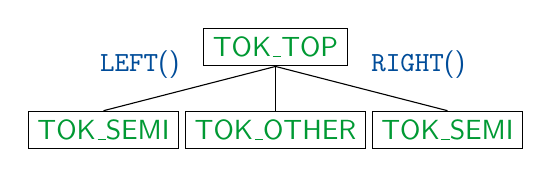
\begin{tikzpicture}[font=\sffamily,thick,level/.style={sibling distance=50mm/#1}]
%\tikzset{text width=5.8em, text centered}
\tikzset{every tree node/.append style={draw}}
\Tree [.\Token{TOP}
         \edge node[auto=right]{\func{LEFT}\fp}; \Token{SEMI}
         %\leftToken{SEMI}
         \Token{OTHER}
         \edge node[auto=left]{\func{RIGHT}\fp}; \Token{SEMI}
         %\leftToken{SEMI} 
         ]
\end{tikzpicture}%}

% Currently we cannot fit much here...
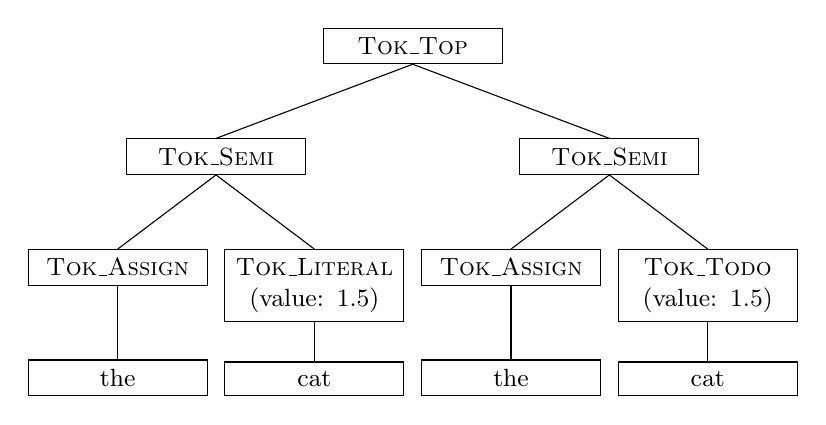
\begin{tikzpicture}
\tikzset{level distance=40pt, sibling distance=6pt, text width=5.8em, text centered}
\tikzset{every tree node/.append style={draw}}
\tikzstyle{every node}=[font=\small]
\Tree [.{{\sc Tok\_Top}}
        [.{{\sc Tok\_Semi}}
          [.{{\sc Tok\_Assign}}
            the
          ]
          [.{{\sc Tok\_Literal} (value: 1.5)} cat ]
        ]
        [.{{\sc Tok\_Semi}}
          [.{{\sc Tok\_Assign}}
            the
          ]
          [.{{\sc Tok\_Todo} (value: 1.5)} cat ]
        ]
      ]
\end{tikzpicture}
}

\section{Code Generation -- producing bytecode}

Code generation is the next step of parsing and is implemented in the file \nasalsourcefile{codegen.c}.  It takes the expression tree generated by the lexer and \nasalsourcefile{parse.c} recursively traverses it to create opcodes -- little ``numbers'' (or an  \type{enum}) that are interpreted by the Nasal Virtual Machine as instructions.  With the exception of blockoids (which have a slightly different structure with up to three children), the token structure that code generation gets is a tree where the most important (highest precedence) tokens are on top, and tokens of lesser- and equal-importance tokens on the sides; laws of grouping are followed as well (like parenthesis and such) by having both left and right children point to the top of the tree for the expression inside of the block.

The example above shows what is really neat about this approach: when it is parsing, say, an assignment operator ($=$), it knows that the left side is going to be a symbol and that the right side can be any type of expression.  Seeing it this way makes much more sense then first seeing the symbol, looking ahead for an assignment, and then hoping the rest of the tokens parse correctly -- that would be a more text-based approach and it is not scalable for complicated syntaxes with oodles of operators with different semantics.

The method used in \nasalsourcefile{parse.c} allows for the minimal-step, maximally-recursive code generator present in Nasal: parsing a mathematical operator is as simple as generating the left and right expressions, and then emitting the correct VM instruction afterwards -- the function handling the mathematical operator does not need to know what lives below the operator, only that it exists.  Each step of the generator (implemented in the \nasalapi{gen\br Expr} function and surrounding static functions) takes the smallest step it can and lets the parse tree work itself out by calling helper functions to handle expressions and expression lists.

Local macros helping with abstraction include:

\begin{enumerate}
\item \localmacro{LEFT(tok)} to get the left-hand branch of a token (i.e. \verb$tok->children$).
\item \localmacro{RIGHT(tok)} to get the right hand branch of a token (i.e. \verb$tok->lastChild$).
\item \localmacro{BINARY(tok)} to check if a token is a binary expression (if there is only two children: \verb$tok->children$ and \verb$tok->lastChild$, and nothing in between, meaning that they reference each other in their \name{next/prev} members).
\end{enumerate}

The low-level workhorses of the code generator are the \nasalapi{emit}\fp\ and \nasalapi{emit\br Immediate}\fp\ functions, which directly write bytecode into the parser structure's codegen pointer.

\begin{lstlisting}[language=C]
static void emit(struct Parser* p, int val)
{
    // Reallocate if necessary
    if(p->cg->codesz >= p->cg->codeAlloced) {
        int i, sz = p->cg->codeAlloced * 2;
        unsigned short* buf = naParseAlloc(p, sz*sizeof(unsigned short));
        for(i=0; i<p->cg->codeAlloced; i++) buf[i] = p->cg->byteCode[i];
        p->cg->byteCode = buf;
        p->cg->codeAlloced = sz;
    }
    // And add our next opcode
    p->cg->byteCode[p->cg->codesz++] = (unsigned short)val;
}
\end{lstlisting}

\begin{lstlisting}[language=C]
static void emitImmediate(struct Parser* p, int val, int arg)
{
    emit(p, val);
    emit(p, arg);
}
\end{lstlisting}

This ``immediate'' value is associated with the opcode and retrieved later in the VM stage.  In general it is just an \type{unsigned short}, but it can mean several things.

Some immediate-mode opcodes refer to the constants table -- this is a chunk in the \type{naCode} which holds scalar constants (string/numeric literals) and code constants (\nasalkeyword{func}\{\} blocks in the code).  These opcodes always need the constants index added when \nasalapi{emit\br Imme\-diate}\fp\ is called, using either \nasalapi{find\br Constant\br Index}\fp\ or a precomputed index, such as returned from \nasalapi{new\br Constant}\fp.  Of this type, there are only these three:
\begin{enumerate}
 \item \OP{PUSHCONST}
 \item \OP{MEMBER}
 \item \OP{LOCAL}
\end{enumerate}

In addition, these two use their immediate value to represent their number of arguments; this is because the VM needs to be able to pop the right amount of arguments from the operand stack:
\begin{enumerate}
\item \OP{FCALL}
\item \OP{MCALL}
\end{enumerate}

And lastly, branching instructions are also immediate-mode; their immediate value refers to the index of the command to jump to.  The specific opcodes are:
\begin{enumerate}
\item \OP{JIFTRUE}
\item \OP{JIFNOT}
\item \OP{JIFNOTPOP}
\item \OP{JIFEND}
\item \OP{JMP}
\item \OP{JMPLOOP}
\end{enumerate}

When jumping backwards, the address is saved away earlier and emmitted with the \Op{Jmp} instruction, but when jumping forwards, the code it is jumping to does not exist yet and therefore its index is not known.  To get around that, there are some functions to handle forward-jumps.  \nasalapi{emit\br Jump} makes a new jump with a dummy index:

\begin{lstlisting}[language=C]
// Emit a jump operation, and return the location of the address in
// the bytecode for future fixup in fixJumpTarget
static int emitJump(struct Parser* p, int op)
{
    int ip;
    emit(p, op);
    ip = p->cg->codesz;
    emit(p, 0xffff); // dummy address
    return ip;
}
\end{lstlisting}

As suggested by the comment, \nasalapi{fix\br Jump\br Target} is what comes along at the desired jump-to point and adds in the correct index:

\begin{lstlisting}[language=C]
// Points a previous jump instruction at the current "end-of-bytecode"
static void fixJumpTarget(struct Parser* p, int spot)
{
    p->cg->byteCode[spot] = p->cg->codesz;
}
\end{lstlisting}

For typical usage, here's a stripped down \nasalapi{gen\br If} example:

\begin{lstlisting}[language=C]
static void genIf(struct Parser* p, struct Token* tif, struct Token* telse)
{
    int jumpNext, jumpEnd;
    genExpr(p, tif->children); // the test
    jumpNext = emitJump(p, OP_JIFNOTPOP);
    genExprList(p, tif->children->next->children); // the body
    jumpEnd = emitJump(p, OP_JMP);
    fixJumpTarget(p, jumpNext);
    if(telse) {
        if(telse->type == TOK_ELSIF) genIf(p, telse, telse->next);
        else genExprList(p, telse->children->children);
    } else {
        emit(p, OP_PUSHNIL);
    }
    fixJumpTarget(p, jumpEnd);
}
\end{lstlisting}

The first jump points to right after the second jump, since \nasalapi{fix\br Jump\br Target} is called after \nasalapi{emit\br Jump} is called the second time.  After the \nasalkeyword{else}\{\} clause is handled, the second jump is made to point after all of that.  The power in this is allowing arbitrary chunks of code (e.g. as emitted from \nasalapi{gen\br Expr\br List}) to be jumped over.

\subsection{Initialization}

Code generation itself is started in \nasalapi{na\br Code\br Gen}\fp\ where the code generation related data structures are allocated and initialized, including:

\begin{enumerate}
\item an \type{naCode}* code object
\item argument list processing
\end{enumerate}

Afterwards, \nasalapi{gen\br Expr\br List}\fp\ is invoked, which in turn recursively invokes itself and \nasalapi{gen\br Expr}\fp\ while traversing the semi-colon-seperated statements in the parse tree, the latter is the primary workhorse of the code generator in that it will recognize and turn tokens into bytecode primitives.

\subsection{Constants Table}

This stores constants used in a function's body, both scalars and code. Implemented during codegen as a \type{naVec} for the purposes of cheap alloc handling, this gets turned into a static table as part of the \type{naCode} structure.  \nasalapi{internConstant}\fp\ is used to return a reference to the existing constant if one already exists; it relies on \nasalapi{newConstant}\fp\ to add the constant if needed.  Code for both (in reverse order of declaration):

\begin{lstlisting}[language=C]
// Interns a scalar (!) constant and returns its index
static int internConstant(struct Parser* p, naRef c)
{
    int i, n = naVec_size(p->cg->consts);
    if(IS_CODE(c)) return newConstant(p, c);
    for(i=0; i<n; i++) {
        naRef b = naVec_get(p->cg->consts, i);
        if(IS_NUM(b) && IS_NUM(c) && b.num == c.num) return i;
        else if(IS_NIL(b) && IS_NIL(c)) return i;
        else if(naStrEqual(b, c)) return i;
    }
    return newConstant(p, c);
}

static int newConstant(struct Parser* p, naRef c)
{
    int i;
    naVec_append(p->cg->consts, c);
    i = naVec_size(p->cg->consts) - 1;
    if(i > 0xffff) naParseError(p, "too many constants in code block", 0);
   return i;
}
\end{lstlisting}

\section{The Code Generation API}
\todo{document the codegen.c APIs?}

\section{Code Generation Examples}
\todo{discuss loops, function calls, methods?}

\section{Virtual Machine: running code}
As mentioned before, the Nasal bytecode gets executed in \nasalsourcefile{code.c} using an infinite interpreter loop with a huge switch/case block in the form of the \func{run}\fp\ function in \nasalsourcefile{code.c}.  This is the ``Virtual Machine'' (VM) of Nasal.  In general, machines take some form of operations (e.g. Nasal bytecode) and execute them based upon other factors, like other inputs, and then produce an output of some kind.  (A \emph{virtual} machine is simply such a machine that is implemented in software not hardware -- e.g. C/C++ code versus circuit boards).  Some of the simplest machines are stack machines; this is what is used for the Nasal VM, stack machines are generally a popular concept, and e.g. also used by Java.  The Nasal stack machine uses two main stacks and \emph{pushes} and \emph{pops} from those stacks.  Each stack is an array of variables with a fixed size -- exceeding this size is an error.  The first stack is where all the opcodes are stored and it is for all purposes of type \type{unsigned short} or \type{int}, since each opcode is part of an enumeration.  This also allows other integers to live on the stack as well (more on this later).  The other stack is made up of \type{naRefs}, which are the ``operands'' that the opcodes operate on.

For most typical opcodes, the VM pops some arguments from the stack -- that is, it takes the top item on the stack and saves it to a variable if needed, then it decrements the top of the stack so that the popped argument ``disappears'' from the stack.  After performing the operation, the VM will push a result back onto the stack -- this does the opposite of popping as it increments the top of the stack and sets the new top item.  Thus pushing makes a ``new'' item on the top of the stack while popping takes one away.  Eventually this change in state cascades down as a result of operations and a useful output is acheived.  While the Nasal VM can do a fair amount of variable-handling operations on its own, \type{naCFunctions} can add more operations (e.g. \func{f\_setsize}\fp) or can provide access to anything accessible from C space, like \func{f\_print}\fp\ and the io library do.

These two stacks live in different places.  The opcode stack lives in the \type{naCode} object under the constants block and is extracted using the \globalmacro{BYTECODE}\fp\ macro defined in \nasalsourcefile{data.h}, which typecasts the \type{naRef} to an \type{unsigned short}* (see \nasalsourcefile[147]{data.h}, line 147).  The ``cursor'' for the bytecode is stored in the current frame's \name{ip} member.  A common operation is then \type{int} \verb$op = $\func{BYTECODE}\verb$(cd)[f->ip++];$ (which is used in \nasalsourcefile{code.c} to retrieve the opcode and/or an argument, implicitly typecasting to an integer).  By this method, the opcode ``stack'' is not a ``true'' stack in the fact that it is immutable (should {\bf not} be changed except using stack operations like push/pop!) and can only move one direction (adds to it during code generation, moves down it during the running of the code).  The other stack -- the one of \type{naRefs} -- is actually a real stack.  The items are stored in the context's \name{opStack} member, which has \localmacro{MAX\_STACK\_DEPTH} number of terms, and its cursor is stored in the \name{opTop} member.  Note that indexing \name{opStack} with the current \name{opTop} index is not a valid operation -- the true top item on the stack is one below is at \verb$STK(1)$ or \verb$ctx->opTop-1$.  There are various helper macros to help out with operations on this stack, like \func{PUSH}\fp\ and \func{POP}\fp\ and in particular \localmacro{STK(n)}, which directly retrieves an item on the stack (where $n=1$ is the top member as previously mentioned, and $n=2$ is the second, etc.).  Note that the \func{STK}\fp\ macro requires manual movement of the \name{opTop} index, i.e. the programmer has to use \verb$ctx->opTop--$ or \verb$ctx->opTop-=2$.  For more info, see code.c, line 246 for \func{PUSH}\fp, and lines 520--523 for the other macros.

Also, there are two other relevant stacks.  The first one is the stack of frames.  Since a function can be called in an overlapping fashion (e.g. a function calling itself recursively, or being called in a multithreaded fashion from different threads), Nasal needs separate places to store information for each separate call.  This stack is made up of \type{struct Frames} and lives in the \name{fStack} member, which has size of \localmacro{MAX\_RECURSION}, and its index is in the \name{fTop} member.  New calls are pushed in at the \name{fTop} index and the current frame is \verb$ctx->fStack[ctx->fTop-1]$ while the first frame is \verb$ctx->fStack[0]$.

\subsection{An example}
To take an example of the VM in action, let's say that we execute this Nasal statement:

\begin{lstlisting}[language=nasal]
var foo = 1.5-0.5;
\end{lstlisting}

This takes and sets the local variable ``foo'' with the result of 1.5 minus 0.5 (code generation does not optimize any).  This would produce a stack of opcodes like this:

\todo{all these examples are neat and important, but tedious and error-prone to create: we should automate the creation of them using our Nasal/LaTex hacks, so that we can dump the stacks to the console and even turn them into nice "stack tables" to be used here}

\begin{verbatim}
Stack of op codes:   Stack of arguments:
[start]              ...      ctx->opTop
OP_PUSHCONST                  [end]
00003
OP_PUSHCONST
00004
OP_MINUS
OP_PUSHCONST
00005
OP_SETLOCAL
...
OP_RETURN
\end{verbatim}

The first two opcodes are \Op{Pushconst}s, which take a constant and pushes it onto the (previosuly empty) stack at the top. This illustrates the fact that each function call starts with a clean stack of operands, and all constants have to be initialized. This particular one points to constant `3', which should hold an \type{naRef} with it's number set to 0.5.  Then we push another number, which will be 1.5.  Then we get this stack:

\begin{verbatim}
Stack of op codes:   Stack of arguments:
...                  ...      ctx->opTop
OP_MINUS             naRef  1.5   STK(1)
OP_PUSHCONST         naRef  0.5   STK(2)
00005                         [end]
OP_SETLOCAL
...
OP_RETURN
\end{verbatim}

The first opcode is \Op{Minus}, which takes the first argument (1.5) and subtracts the second (0.5) and places the result (1.0) where the second used to be, then decrements the top of the stack.  The stack now looks like this:

\begin{verbatim}
Stack of op codes:   Stack of arguments:
...                  ...      ctx->opTop
OP_PUSHCONST         naRef  1.0   STK(1)
00004                         [end]
OP_SETLOCAL
...
OP_RETURN
\end{verbatim}

Now we see \Op{Pushconst} and a number after it.  This push operation takes an argument of type \type{int} from the stack of opcodes, not \type{naRefs}, and retrieves the constant \type{naRef} stored at the specified index in the constants block of the currently executing code using the \localmacro{CONSTARG}\fp\ macro \citesourcefile[520]{code.c}.  During code generation, this constant is saved away inside of the code's constant block for each required lvalue, and this opcode pushes the correct one onto the stack -- which should be a \type{naRef} representing ``foo'' and is pushed in before the result of the \Op{Minus}, setting us up for the next step:

\begin{verbatim}
Stack of op codes:   Stack of arguments:
...                  ...      ctx->opTop
OP_SETLOCAL          naRef  foo   STK(1)
...                  naRef  1.0   STK(2)
OP_RETURN                     [end]
\end{verbatim}

We finally get to \Op{Setlocal}, which sets a local variable (i.e. one using the `var' keyword) to a value.  It takes the first argument on the stack as the lvalue (symbolic name) of the variable and the second as the value to set it to.  In this case, we see those are ``foo'' and 1, respectively, and so the variable foo correctly gets set to 1.  Note that this operation does not explicitly ``return'' anything, i.e. it does not push a `result', but it does have the implicit return of the value set, since that is the last argument left on the stack (since the \Op{Setlocal} operation only moves down 1 on the stack).  This illustrates an interesting feature of Nasal: it always has its current working state and every operation returns \emph{something}.  We will see this in action in the next paragraph.

\begin{verbatim}
Stack of op codes:   Stack of arguments:
...                  ...      ctx->opTop
OP_RETURN            naRef  ??    STK(1)
\end{verbatim}

We execute some more statements in between and eventually get to a return opcode -- this is required otherwise the Nasal VM will get stuck in an infinite loop and possibly do some very weird things.  Anyways, sometimes this return is implicit and is synthesized by the code generation, if so it returns the first argument on the stack -- remember how we called it the ``current working state''? An equivalent expression that makes this return explicit goes like so:

\begin{lstlisting}[language=Nasal]
return (...);
\end{lstlisting}

Substitue the last expression you want to execute into the parentheses and you are set.  A great mistake would be to say ``Oh, I just need to type return-$\langle$semicolon$\rangle$ and I'll be set.''  This is incorrect, since code generation makes an \Op{Pushnil} before any return statement like this:

\begin{lstlisting}[language=Nasal]
return (...);
\end{lstlisting}

Thus it would really return nil, not the last expression that was evaluated.  See line 631 of \nasalsourcefile[631]{codegen.c} for more information.

\todo{we should generalize this, turn it into a command and use it as a template for LaTex-based stack diagrams that can be emitted from Nasal directly}
\usetikzlibrary{shapes.multipart} 
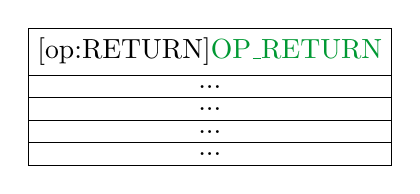
\begin{tikzpicture}[stack/.style={rectangle split, rectangle split parts=#1,draw, anchor=center, fill=white}]
  \node[stack=5]  {
    \nodepart{one}\OP{RETURN}
    \nodepart{two}...
    \nodepart{three}...
    \nodepart{four}...
    \nodepart{five}...
  };
\end{tikzpicture}

\subsection{VM Operators/Opcodes}
Here is a semi-comprehensive list of all the operators and their functions.

\subsubsection{Unary operators}
Operators that modify STK(1) in place:
\begin{description}
    \item \OP{NOT} \label{op:NOT}\label{op:Not} Boolean inverse (i.e. \verb$!a$, $\neg a$).
    \item \OP{NEG} \label{op:NEG}\label{op:Neg} Additive inverse (i.e. \verb$-a$, $-a$).
\end{description}

\subsubsection{Binary operators}
Operators that pop two arguments and push a result:
\begin{description}
    \item \OP{PLUS} \label{op:PLUS} \label{op:Plus} Addition (i.e. \verb$a+b$, $a + b$).
    \item \OP{MINUS}\label{op:MINUS}\label{op:Minus} Subtraction (i.e. \verb$a-b$, $a - b$).
    \item \OP{MUL}  \label{op:MUL} \label{op:Mul} Multiplication (i.e. \verb$a*b$, $a\times b$).
    \item \OP{DIV}  \label{op:DIV} \label{op:Div} Division (i.e. \verb$a/b$, $a\div b$).
    \item \OP{CAT}  \label{op:CAT} \label{op:Cat} Concatenate either two vectors or two strings (i.e. \verb$a~b$).
    \item \OP{LT}   \label{op:LT} \label{op:Lt} Strictly less-than (i.e. \verb$a<b$, $a < b$).
    \item \OP{GT}   \label{op:GT} \label{op:Gt} Strictly greater-than (i.e. \verb$a>b$, $a > b$).
    \item \OP{LTE}  \label{op:LTE} \label{op:Lte} Less-than-or-equal-to (i.e. \verb$a<=b$, $a\leq b$).
    \item \OP{GTE}  \label{op:GTE} \label{op:Gte} Greater-than-or-equal-to (i.e. \verb$a>=b$, $a\geq b$).
    \item \OP{EQ}   \label{op:EQ} \label{op:Eq} Equality or equivalence (i.e. \verb$a==b$, $a\equiv b$; tests for numerical esuality if possible and acts recursively on hashes and vectors besides comparing pointers).
    \item \OP{NEQ}  \label{op:NEQ}\label{op:Neq} Non-equality/equivalence (i.e. \verb$a!=b$, $\neg(a\equiv b)$).
\end{description}

\subsubsection{Push and/or pop operations}
Operations that push or pop a \type{naRef} directly from the stack:
\begin{description}
    \item \OP{POP} \label{op:POP} \label{op:Pop} Pop one \type{naRef} off of the stack (actually, it just moves the top of the stack down one).
    \item \OP{DUP} \label{op:DUP} \label{op:Dup} Push a duplicate of the top item.
    \item \OP{DUP2}\label{op:DUP2}\label{op:Dup2} Push duplicates of the top two items (e.g. $a, b$ becomes $a', b', a, b$).
    \item \OP{PUSHONE}  \label{op:PUSHONE}\label{op:Pushone} Push a \type{naRef} `1'.
    \item \OP{PUSHZERO} \label{op:PUSHZERO}\label{op:Pushzero} Push a \type{naRef} `0'.
    \item \OP{PUSHNIL}  \label{op:PUSHNIL}\label{op:Pushnil}  Push a \func{naNil}\fp.
    \item \OP{PUSHEND}  \label{op:PUSHEND}\label{op:Pushend} Push an \func{endToken}\fp.
    \item \OP{PUSHCONST}\label{op:PUSHCONST}\label{op:Pushconst} Take an integer argument from the {\bf opcode} stack then retrieve and push the constant found at that index in the code's constants block.  See the \globalmacro{CONSTARG}\fp\ macro, line 520 in \nasalsourcefile[520]{code.c}, for more details.  Also note that if the constant is a \type{naCode} object (inside of its \type{naRef} shell), then it gets bound to the current context/frame via \func{bindFunction}\fp\ (which turns it into a \type{naFunc}).
    \item \OP{NEWVEC}   \label{op:NEWVEC}\label{op:Newvec}  Push a new vector.
    \item \OP{NEWHASH}  \label{op:NEWHASH}\label{op:Newhash} Push a new hash.
\end{description}

\subsubsection{Jump operations}
\todo{should this be renamed BRANCHING and should we differentiate here between unconditional and conditional branching ?}
Operations that jump within either stack:
\begin{description}
    \item \OP{JMP}    \label{op:JMP}\label{op:Jmp} Execute a non-conditional jump to the bytecode index specified by the next item on the opcode stack (i.e. an integer one).
    \item \OP{JMPLOOP}\label{op:JMPLOOP}\label{op:Jmploop} Same, but execute \func{naCheckBottleneck}\fp\ first.
    \item \OP{JIFTRUE}\label{op:JIFTRUE}\label{op:Jiftrue} Jump if the top \type{naRef} on the stack is true.  Does {\it not} pop from the stack!
    \item \OP{JIFNOT} \label{op:JIFNOT}\label{op:Jifnot} Same, but jumps if false.
    \item \OP{JIFNOTPOP}\label{op:JIFNOTPOP}\label{op:Jifnotpop} Same as \Op{Jifnot} but \emph{does} pop from the stack.
    \item \OP{JIFEND} \label{op:JIFEND}\label{op:Jifend} Jumps if the top \type{naRef} is an \func{endToken}\fp\ (i.e. the pointer equals \verb$($\type{void}*\verb$)1$).  Pops only if it is an \func{endToken}\fp.
    \item \OP{MARK}   \label{op:MARK}\label{op:Mark} Pushes a mark (the current size of the \type{naRef} stack) onto the mark stack.
    \item \OP{UNMARK} \label{op:UNMARK}\label{op:Unmark} Pops off a mark and discards it.
    \item \OP{BREAK}  \label{op:BREAK}\label{op:Break}   Takes and restores a mark position.
    \item \OP{BREAK2} \label{op:BREAK2}\label{op:Break2} Same, but pops it off instead of leaving it.
\end{description}

\subsubsection{Function calls}
These opcodes either call a \type{naCCode} or push another stack frame for a \type{naCode} call.  The number of arguments is compiled during code generation and is thus fixed.  By default, the top \name{nargs} on the stack are used as the arguments, another \type{naRef} is popped off as the function, and for method calls, another is popped off for the `me' reference.  For named arguments, there is only 1 argument that is taken from the stack, which becomes the \name{locals} hash for the new frame, otherwise the \name{locals} are made by the \func{setupArgs}\fp\ function.
\begin{description}
    \item \OP{FCALL} \label{op:FCALL}\label{op:Fcall} A basic function call.
    \item \OP{MCALL} \label{op:MCALL}\label{op:Mcall} A method call -- sets the `me' symbol.
    \item \OP{FCALLH}\label{op:FCALLH}\label{op:Fcallh} A function call with named arguments (the `H' is probably for ``hash-like'').
    \item \OP{MCALLH}\label{op:MCALLH}\label{op:Mcallh} A method call with named arguments.
\end{description}

\subsubsection{Set methods}
These methods set a variable and usually leave the value that was set on the stack, thus in most cases where you want to set something and don't care about the return, these should be followed by \Op{Pop}.
\begin{description}
    \item \OP{SETLOCAL} \label{op:SETLOCAL}\label{op:Setlocal} Set the local variable named by STK(1) to the value given by STK(2).
    \item \OP{SETSYM}   \label{op:SETSYM}\label{op:Setsym} Like \Op{Setlocal} but tries to find the variable in successive namespaces (i.e. each \verb$func->next$ in turn).  If it is not found there, place it in the locals.
    \item \OP{SETMEMBER}\label{op:SETMEMBER}\label{op:Setmember} STK(1) is the name of the member, STK(2) is the hash, and STK(3) is the value.
    \item \OP{INSERT}   \label{op:INSERT}\label{op:Insert} Like \Op{Setmember} but more generic for the case of vectors as well (i.e. \verb$hashvec[index]$ versus \verb$hash.member$).
    \item \OP{HAPPEND}  \label{op:HAPPEND}\label{op:Happend} Another hash set but this time with the arguments in a funny order: STK(1) is the value to set, STK(2) the name, and STK(3) the hash.
\end{description}

\subsubsection{Symbol ``get'' methods}

\begin{description}
    \item \OP{LOCAL}  \label{op:LOCAL}\label{op:Local} Takes a constant argument and pushes 
    \item \OP{MEMBER} \label{op:MEMBER}\label{op:Member} Retrieve a member from STK(1) with the name given by a \localmacro{CONSTARG}\fp.  Recurses into the parents vector if necessary.  This is unique -- no other function goes into the parents vector!
\end{description}

\subsubsection{Miscellaneous}
Other opcodes:
\begin{description}
    \item \OP{XCHG}   \label{op:XCHG}\label{op:Xchg}  Swap the top two items on the stack.
    \item \OP{XCHG2}  \label{op:XCHG2}\label{op:Xchg2} Swap the top three items on the stack (i.e. first becomes third and the two others get shifted `up' in the stack, thus a 1-2-3 order gets converted to a 2-3-1 order).  An \Op{Xchg2} followed by an \Op{Xchg} results in a total reversing (i.e. 3-2-1) and \Op{Xchg} followed by an \Op{Xchg2} results in a swap of the lower two items (i.e. 1-3-2).
    \item \OP{EACH}   \label{op:EACH}\label{op:Each} Works like a vector get: STK(1) is the index and STK(2) is the vector; it then increments the index and pushes the result.
    \item \OP{INDEX}  \label{op:INDEX}\label{op:Index} Same, but pushes a copy of the index instead of the variable at that position in the vector.
    \item \OP{UNPACK} \label{op:UNPACK}\label{op:Unpack} Take the contents of the vector on the top of the stack and push its contents one-by-one for the number of times specified by the argument on the opccode stack.
    \item \OP{RETURN} \label{op:RETURN}\label{op:Return} If this is the top of the call stack (i.e. \name{fTop} is 1) then it returns from the \func{run}\fp\ function with the value of STK(1), else it resets to the next call up the stack setting the new STK(1) with the value of the old STK(1).
\end{description}

\subsection{Stack Frames}
Stack frames are essential to running a programming language.  Functions call other functions, and their data must be stored on a stack.  In Nasal, each \type{struct Context} object has a stack of frames in its \type{struct Frame} \name{fStack[]} member, whose top is stored in the \type{int} \name{fTop} member.  The definition of each element is:
\begin{lstlisting}[language=C]
struct Frame {
    naRef func;
    naRef locals;
    int ip;
    int bp;
};
\end{lstlisting}

The \name{func} member stores the \type{naFunc} that created the Frame.  The \name{locals} member is a new hash that is loaded with the arguments to the function and is used as the ``running namespace''; it is discarded when the function returns, unless saved by some means (either making a \nasalkeyword{func}\{\} that is findable by the GC or using the \func{caller}\fp\ API).  Thus, despite many calls to the same function, especially in recursion, each invocation will safely run in its own, separate ``workspace'' and will not interfere with other calls of the same function.  The \name{ip} and \name{bp} members refer to the position in the opcode (instruction pointer and base pointer) and \type{naRef} stacks, respectively.  The former begins at 0 while the latter is equivalent to the \verb$ctx->opFrame$ at the time and is used to pop \verb$ctx->opFrame$ back to its old value, so that the function can access its own data on that stack again.

As a function call is executed, its frame is pushed onto the stack at the current \name{fTop} index, which is then pushed up one.  Thus the frame of the currently executing code is \verb$ctx->fStack[ctx->fTop-1]$.

The relationship of of the operand stack with function calls is rather weird.  All functions on a context's call stack end up using the same operand stack, and they all have access only to the top of it -- specifically they should only access those that they pushed themselves.  When a function call is done, any of its data on the stack gets popped by setting \verb$ctx->$\br\verb$opFrame$\br\verb$ = $\br\verb$ctx->$\br\verb$fStack$\br\verb$[ctx->fTop$\br\verb$-1]$\br\verb$.bp$, its return gets pushed, and now the old function can use its old operands, with the return now added on top.

\comment{
% stack frame example taken from: https://gitorious.org/tikz-goodies/tikz-goodies/blobs/0dffd069488fc812050e6ce5513736e83eaa666b/drawstack/stack-example.tex
% also see: ftp://ftp.dante.de/tex-archive/macros/latex/contrib/drawstack/stack-example.pdf
\todo {generalize this, style it for Nasal and then emit it directly via the interpreter}
\begin{drawstack}
  \startframe
  \cell{First cell}
  \cell{Second cell}
  \finishframe{Some stack frame}
  \cell{Not interesting}
  \startframe
  \cell{Next stack frame}
  \cell{Next stack frame}
  \finishframe{Another stack frame}
\end{drawstack}

\begin{enumerate}
  \item \url{http://stackoverflow.com/questions/10057443/explain-the-concept-of-a-stack-frame-in-a-nutshell}
  \item \url{http://www.cs.umd.edu/class/sum2003/cmsc311/Notes/Mips/stack.html}
  \item \url{http://en.wikibooks.org/wiki/X86_Disassembly/Functions_and_Stack_Frames}
  \item \url{http://en.wikipedia.org/wiki/Stack_frame#Structure}
  \item \url{http://www.dirac.org/linux/gdb/02a-Memory_Layout_And_The_Stack.php}
  \item \url{http://blog.morrisjohns.com/javascript_closures_for_dummies.html}
  \item \url {http://mark-story.com/posts/view/picking-up-javascript-closures-and-lexical-scoping}
\end{enumerate}
}

\todo{we can inspect stack frames using helpers in findFrame(), see naGetSourceFile() and naGetLine() for examples}

\section{Garbage Collection}
\subsection{Mark \& Sweep}
When using a mark-and-sweep collector, unreachable objects are not immediately reclaimed.  Instead, garbage is allowed to accumulate until all available memory has been exhausted.  When that happens, the execution of the program is suspended temporarily while the mark-and-sweep algorithm collects all the garbage.  Once all unreferenced objects have been reclaimed, the normal execution of the program can resume.

Obviously, the main disadvantage of the mark-and-sweep approach is the fact that that normal program execution is suspended while the garbage collection algorithm runs.  In particular, this can be a problem in a program that must satisfy real-time execution constraints (like a flight simulator).  For example, an interactive application that uses mark-and-sweep garbage collection becomes unresponsive periodically.

The mark-and-sweep algorithm is called a tracing garbage collector because is traces out the entire collection of objects that are directly or indirectly accessible by the program.  The objects that a program can access directly are those objects which are referenced by local variables on the processor stack as well as by any static variables that refer to objects.  In the context of garbage collection, these variables are called the roots.  An object is indirectly accessible if it is referenced by a field in some other (directly or indirectly) accessible object.  An accessible object is said to be live.  Conversely, an object which is not live is garbage.

The mark-and-sweep algorithm consists of two phases: In the first phase, it finds and marks all accessible objects.  The first phase is called the mark phase.  In the second phase, the garbage collection algorithm scans through the heap and reclaims all the unmarked objects.  The second phase is called the sweep phase.

Nasal's implementation of \nasalapi{sweep}\fp\ (called \nasalapi{reap}\fp) works such that it is always executed for a handful of different type-specific memory pools.  In addition, it also makes sure to allocate new memory if required.

\subsection {Nasal Memory Pools}
A memory pool is basically a preallocated region of memory, which is dynamically resized as required.  The Nasal GC works such that it manages a handful of global memory pools for all native Nasal types (strings, functions, vectors, hashes etc). At the moment, the hard coded defaults ensure that 25--50\% of additional object "slots" (memory blocks) are kept available during each execution of reap().

Whenever new memory is requested to create a new type (such as a vector or a string), the available memory in the corresponding pool will be checked, reachable objects will be marked, and dead objects will be removed from all pools using a mark/sweep collector, new memory blocks will be allocated if necessary.  All of this happens atomically, i.e. single-threaded, in a ``stop-the-world'' fashion.

All Nasal memory pools are implemented using memory blocks, a memory block is implemented as a singly linked list.  Each block contains a field to store its size, a pointer to the allocated memory, and another pointer to the next block.

\begin{lstlisting}[language=C]
struct Block {
    int   size; // size of the block 
    char* block; // pointer to the memory region
    struct Block* next;	// pointer to the next block
};
\end{lstlisting}

For each of the 7 Nasal data types, there is a separate storage pool used, declared as part of the "Globals" structure.  As can be seen, each storage pool is addressed by its enum index (0..6):
\begin{lstlisting}[language=C]
enum { T_STR, T_VEC, T_HASH, T_CODE, T_FUNC, T_CCODE, T_GHOST, NUM_NASAL_TYPES };
\end{lstlisting}

The 7 storage pools are declared in \nasalsourcefile{code.h} as part of the "Globals" structure:

\begin{lstlisting}[language=C]
struct Globals {	
    // Garbage collecting allocators:
    struct naPool pools[NUM_NASAL_TYPES];
    int allocCount;
    // Dead blocks waiting to be freed when it is safe
    void** deadBlocks;
    int deadsz;
    int ndead;
//...
};
\end{lstlisting}

New memory blocks are allocated using \nasalapi{newBlock}\fp\ and the memory is initialized with 0:

\begin{lstlisting}[language=C]
static void newBlock(struct naPool* p, int need)
{
    int i;
    struct Block* newb;
    if(need < MIN_BLOCK_SIZE) need = MIN_BLOCK_SIZE;
    // allocate a new Block
    newb = naAlloc(sizeof(struct Block));
    // initialize the Block
    newb->block = naAlloc(need * p->elemsz); // number of elements * size of element
    newb->size = need; // set block size 
    // memory blocks are circular linked lists: 
    newb->next = p->blocks;
    p->blocks = newb;
    naBZero(newb->block, need * p->elemsz);

    if(need > p->freesz - p->freetop) need = p->freesz - p->freetop;
    p->nfree = 0;
    p->free = p->free0 + p->freetop;
    // mark all new blocks as unreachable and add them to the pool's free list
    for(i=0; i < need; i++) {
        // initialize each new new memory blocks by setting up an naRef (the container for all Nasal references) 
        struct naObj* o = (struct naObj*)(newb->block + i*p->elemsz);
        o->mark = 0;
        p->free[p->nfree++] = o;
    }
    p->freetop += need;
}
\end{lstlisting}

\section{Error and Exception Handling}
\todo{To be written,explain setjmp, longjmp,naRuntimeError, naParseError}
\subsection{Parser error handling}
This information is relevant to \nasalsourcefile{lex.c}, \nasalsourcefile{parse.c}, and \nasalsourcefile{codegen.c}.

If an error occurs, often relevant information is lacking as there is no ``state'' of the generator, so most errors end up saying ``parse error'' and give you a line number, instead of what could be helpful information such as ``inside a foreach loop, this error occured''.

\subsection{VM error handling}
\subsection{Exception handling via \func{call}\fp}

\part{Examples and Existing Work}
\section{The Nasal Standard Library}
\todo{document lib.c, math.c, etc.}

\section{Multithreading Support}
\todo{document threadlib.c}

\section{Nasal bindings}
\subsection {SQLite}
\subsection {PCRE (regex)}
\subsection {Cairo}
\subsection {Gtk}
\subsection {OpenCL}

%\section{Sandboxing} %(import etc)

\section{Embedding Nasal}
\todo{Look at: nasal-bin.c, AlgoScore, FlightGear's FGNasalSys}
\subsection{Basic Nasal Integration Example}
\begin{enumerate}
  \item create a new context using \nasalapi{naNewContext}\fp
  \item parse the code using \nasalapi{naParseCode}\fp
  \item create the standard namespace using \nasalapi{naInit\_std}\fp
  \item add any custom symbols using \nasalapi{naAddSym}\fp\ (optional)
  \item add other required bindings/libraries (optional)
  \item use \nasalapi{naCall}\fp\ to call the code in the namespace
  \item do error checking using \nasalapi{naGetError}\fp
\end{enumerate}

\begin{lstlisting}[language=C]
// A Nasal extension function (prints its argument list to stdout)
static naRef print(naContext c, naRef me, int argc, naRef* args)
{
    int i;
    for(i=0; i<argc; i++) {
        naRef s = naStringValue(c, args[i]);
        if(naIsNil(s)) continue;
        fwrite(naStr_data(s), 1, naStr_len(s), stdout);
    }
    return naNil();
}
\end{lstlisting}

\subsection{Nasal Integration in FlightGear}
% Also see: http://plausible.org/nasal/flightgear.html
In FlightGear, Nasal is added as a \type{SGSubsystem} in the form of the \name{FGNasalSys} class in \src{\$FG\_SRC}/Scripting/NasalSys.cxx, which is mainly responsible for initializing the interpreter at the moment, as most runtime code is invoked through callbacks that are run via timers and listeners.  It notably introduces FlightGear-specific extension functions, like \func{setlistener}\fp/\func{removelistener}\fp, \func{settimer}\fp, and \func{systime}\fp\ functions, and a new area of development is exposing C++ classes and alternative Nasal APIs via ghosts, like the \func{maketimer}\fp\ function does.

\subsubsection{Initialization}
At the moment, \name{FGNasalSys} loads all the Nasal code currently.  This will hopefully be changed in the future to allow a Nasal script to do all of the loading, making it a more flexible and transparent process, which is important to those who do not compile from source or understand that source but need to know how things work.

Initialization is a big part of running Nasal code in FlightGear and most Nasal libraries/subsystems get loaded this way.  But to keep running intermittently, to provide an alternative method of loading, or to run a Nasal ``action'' script, there are three other ways to run Nasal in FlightGear: timers, listeners, and bindings.
\subsubsection{Timers}
Timers can be used to repetively run bits of code in a loop, somewhat like a proper subsystem in FlightGear, to delay a response to something, or to distrubute work across frames.  \func{settimer}\fp\ is mainly used for this right now, and it simply registers a function to be run after a certain amount of time -- this is checked every frame, and so at maximum it can only run at frame rate.  To run in a loop, the callback must re-register itself in a new timer, which is inefficient.  Recently, \func{maketimer}\fp\ was introduced, which returns a Nasal ghost that is a virtual C++ timer object.  This timer can be stopped, (re-)started, and told to run at a certain interval (solving the need to reregister a timer), or to just run once (like \func{settimer}\fp\ does, though \func{maketimer}\fp\ objects can be reused).  These both illustrate how to constantly run code in FlightGear, and this can be very useful though being limited to the frame rate.
\subsubsection{Listeners}
Another solution to looping is hooking a Nasal callback to a property that is called by some subsystem updating at a potentially higher rate -- like the rate of the underlying flight dynamics model (FDM).  These callbacks are called listeners, and for long-standing reasons they may not work with all properties created by C++ code, but there are some places where they are applicable.  Other uses are waiting for a user input (like adjusting a preference, which may require 3D objects or even Nasal modules to be loaded or unloaded), communicating between systems, receiving direct input from C++ or other languages interfacing with FlightGear, and more.  In the future, all Nasal modules other than necessary libraries might be loaded from listeners, as they provide a convient way to run Nasal code that transcends all languages in FlightGear by using the property tree.
\subsubsection{Bindings/FGCommands}
Bindings are the third and final way to run code.  FlightGear has a core set of commands -- called fgcommands -- that interact with their caller via the property tree and can be executed from both C++ and Nasal (via the \func{fgcommand}\fp function in Nasal).  These are often wrapped in ``bindings'', which are property nodes that store the name of their command and arguments to the command side-by-side.  One of these commands is ``nasal'', which executes a Nasal snippet in a ``script'' node.  Other commands provide access to C++ functionality, such as the flight plan.  Nasal can actually register its own fgcommands, so Nasal code can even be registered to run via bindings that do not use the ``nasal'' command.

One of the exciting things about bindings is that they are prevalent in many areas of FlightGear.  In particular, they are often used to handle user input (joystick and mouse events and ``pick'' animations on 3D objects) and can be incorporated as elements of other systems, like checklists that can be ``run'' by executing sequential bindings.  These three parts of FlightGear, timers, listeners, and bindings, allow for a big diversity in how Nasal code can be executed within FlightGear.  It also illustrates well what they have done with integrating Nasal into its core -- perhaps someday achieving the dream of using Nasal and C/C++ side by side.

\section{Nasal Maintenance}
If Nasal is not maintained well and code bases around it evolve too much, then it might become a broken part of whatever it is integrated into, or even being broken by itself.  When integrating Nasal into a new place, developing infrastructure to cement Nasal and the host application together will be needed, and one even might want to extend core Nasal functionality.  This section aims to teach how some of these tasks can be done.
\todo{to be written}
\subsection{Adding a new Token}
\subsection{Adding a new OP code}
\subsection{Adding a new binary operator}
\subsection{Adding a new loopoid}
\subsection{Adding a new extension function}

\section{Known Bugs \& Issues}
\todo{see FIXMEs, TODO in source code}

\section{Maintenance Examples}
Some ideas (brainstorming)
\begin{enumerate}
 \item iterating through hashes (Philosopher; done)
 \item serialize/unserialize functions
 \item json support
 \item native tasking primitives
 \item DbC: preconditions/postconditions
 \item protected types(via hashes) with implicit locking
 \item do\{\}while() construct or other loopoid (Philosopher)
 \item custom typing
 \item list comprehension
\end{enumerate}

% only add sections here which are not just brainstorming, but for which we have actual code/examples

\subsection{Perl's Spaceship Operator}
See \url{http://wiki.flightgear.org/How_to_add_a_new_binary_operator_to_Nasal} for the full example.

\subsection{Slicing Strings}
Currently, Nasal only supports slicing vectors, not strings.  Let's say that we want the ability to slice strings as well; how would we go about adding this?  First we want to consider what stage of Nasal will be affected: parsing (\nasalsourcefile{parse.c}, \nasalsourcefile{codegen.c}) or running (\nasalsourcefile{code.c})?  It's obvious that since the type of the sliced variable is a runtime property, we will only be editing \nasalsourcefile{code.c}, since anything before that has no knowledge of the types of a variable -- right?  Well I thought so too, but then I looked more closely and saw that \nasalsourcefile{codegen.c} actually pushes a new vector when it sees a slice.  This is an optimization that obviously does not work well with strings, and so I introduced a new opcode to push a slice of the appropriate type -- I called it \textcolor{opcode}{\sc Op\_Newslice}.

\subsection{Tom's String Methods}


\section{VM Extensions}
\todo{Hooray is currently playing around with a bunch of related branches}
\subsection{Dumping internal data structures}
\subsection{Implementing support for parser hooks}
\subsection{Implementing debugging support via VM hooks and custom opcodes}
\comment{breakpoint on call, breakpoint on read/write, conditional breakpoints}
\subsection{Implementing instrumentation/profiling support via codegen hooks}
\subsection{Implementing a bytecode optimizer via VM hooks}
% Writing a simple peephole optimizer
% www.stanford.edu/class/archive/cs/cs143/cs143.1112/materials/lectures/lecture14.pdf
% www.d.umn.edu/~rmaclin/cs5641/Notes/L19_CodeGenerationI.pdf
% inst.eecs.berkeley.edu/~cs164/sp06/lectures/lecture15cgen-6.pdf
% www.complang.tuwien.ac.at/papers/maierhofer%2526ertl97.ps.gz

\subsection{Implementing RAII support via VM events}
\subsection{Exposing GC behavior to Nasal space}

\subsection{Implementing a VM debugger}
\begin{enumerate}
 \item breakpoints (via special opcodes or setjmp exceptions)
 \item stepping
 \item interactive, bash-style interface to stepping/executing code and viewing the state of the VM. Could also be useful to have a ``Nasal explorer'' as well. FGCanvas too, maybe?
\end{enumerate}




\section{Debugging Nasal}
\comment{document usage of gdb, valgrind and debugging libs here}
\todo{see various helpers in debug.c and contrib/int-nasal.c}
\subsection{Dumping Tokens}
\subsection{Dumping the Parse Tree}
\subsection{Dumping Bytecode}
\subsection{Dumping Opcode/Operand Stacks}
\subsection{Dumping Stack Frames}
\subsection{Dumping GC State}

\section{Nasal Syntax}
\todo{A guide to the syntax of Nasal, loopoids, expressions, etc.}


\end{document}

